\documentclass[twoside,a4paper,11pt]{article}
\setlength{\oddsidemargin}{0.25 in}
\setlength{\evensidemargin}{-0.25 in}
\setlength{\topmargin}{-0.6 in}
\setlength{\textwidth}{6.5 in}
\setlength{\textheight}{8.5 in}
\setlength{\headsep}{0.75 in}
\setlength{\parindent}{0 in}
\setlength{\parskip}{0.1 in}

%
% ADD PACKAGES here:
%
\usepackage[utf8]{inputenc} %for UTF8-extended encoding
\usepackage{amsmath,amsfonts,amssymb,graphicx,mathtools,flexisym}
\usepackage{caption} %for figures and labels captions
\usepackage{pbox} %to break the cell text in tables
\usepackage[skins,theorems]{tcolorbox} %to create color boxes for examples and recap

\usepackage[colorinlistoftodos,prependcaption,textsize=tiny]{todonotes}
\usepackage{tikz}
\usetikzlibrary{patterns,3d,calc}

\captionsetup{labelsep=space}
%
% The following commands set up the lecnum (lecture number)
% counter and make various numbering schemes work relative
% to the lecture number.
%
\newcounter{lecnum}
\renewcommand{\thepage}{\thelecnum-\arabic{page}}
\renewcommand{\thesection}{\thelecnum.\arabic{section}}
\renewcommand{\theequation}{\thelecnum.\arabic{equation}}
\renewcommand{\thefigure}{\thelecnum.\arabic{figure}}
\renewcommand{\thetable}{\thelecnum.\arabic{table}}

%
% The following macro is used to generate the header.
%
\newcommand{\lecture}[5]{
   \pagestyle{myheadings}
   \thispagestyle{plain}
   \newpage
   \setcounter{lecnum}{#1}
   \setcounter{page}{1}
   \noindent
   \begin{center}
   {\bf COVENTRY UNIVERSITY}
   \framebox{
      \vbox{\vspace{2mm}
    \hbox to 6.28in { {\bf 208MED: Mechanics
	\hfill Spring 2019} }
       \vspace{4mm}
       \hbox to 6.28in { {\Large \hfill Lecture #1: #2  \hfill} }
       \vspace{2mm}
       \hbox to 6.28in { {\textsl{#3} \hfill \texttt{#4}} }
      \vspace{2mm}}
   }
   \end{center}
   \markboth{Lecture #1: #2}{Lecture #1: #2}

%   {\bf Note}: {\it LaTeX template courtesy of UC Berkeley EECS dept.}

   {\bf Disclaimer}: {\it These notes have not been subjected to the
   usual scrutiny reserved for formal publications.  They may be distributed
   outside this class only with the permission of the instructor.}
   \vspace*{4mm}
}

% **** IF YOU WANT TO DEFINE ADDITIONAL MACROS FOR YOURSELF, PUT THEM HERE:


\begin{document}
%FILL IN THE RIGHT INFO.
%\lecture{**LECTURE-NUMBER**}{**DATE**}{**LECTURER**}{**SCRIBE**}
\lecture{03}{Torsion and transverse shear}{Dr. Arnaldo Delli-Carri}{ac4213@coventry.ac.uk}
%\footnotetext{These notes are partially based on those of R. C. Hibbeler}

\tableofcontents

% **** YOUR NOTES GO HERE:

\section{Torsion}
\emph{Torque} is a moment that tends to twist a member about its longitudinal axis. Its effect is of primary concern in the design of drive shafts used in vehicles and machinery, and for this reason it is important to be able to determine the stress and the deformation that occur in a shaft when it is subjected to torsional loads. We can physically illustrate what happens when a torque is applied to a circular shaft by considering the shaft to be made of a highly deformable material such as rubber. When the torque is applied, the longitudinal grid lines originally marked on the shaft, Fig. \ref{fig:Torsion}a, tend to distort into a helix, Fig. \ref{fig:Torsion}b, that intersects the circles at equal angles. Also, all the cross sections of the shaft will remain flat: that is, they do not warp or bulge in or out—and radial lines remain straight and rotate during this deformation. Provided the angle of twist is small, then the length of the shaft and its radius will remain practically unchanged.

\begin{figure}[htb]
\centering
\begin{tikzpicture}[y={(0cm,1cm)},x={(1cm,-0.5cm)}, z={(-1cm,-0.5cm)}]
\draw[->] (-5,0,0) -- +(0,1.5,0) node[above]{$y$};
\draw[->] (-5,0,0) -- +(0,0,1.5) node[above]{$z$};
\foreach \x in {-5,-4.8,...,-0.2} {
\draw[canvas is zy plane at x=\x,fill=cyan!50] (0,0) circle (1cm);
}
\foreach \a in {-50,-40,...,120}{
\draw (0,{cos(\a)},{sin(\a)}) -- +(-5,0,0);
}
\draw[thick,red] (0,{cos(20)},{sin(20)}) -- +(-5,0,0);
\draw[canvas is zy plane at x=0,fill=cyan!50] (0,0) circle (1cm);
\draw[->] (0,0,0) -- +(1,0,0) node[above]{$x$};

\begin{scope}[xshift=8cm]
\draw[->] (-5,0,0) -- +(0,1.5,0) node[above]{$y$};
\draw[->] (-5,0,0) -- +(0,0,1.5) node[above]{$z$};
\foreach \x in {-5,-4.8,...,-0.2} {
	\draw[canvas is zy plane at x=\x,fill=cyan!50] (0,0) circle (1cm);
}
\foreach \a in {-50,-40,...,120}{
	\draw (-5,{cos(\a)},{sin(\a)}) -- (0,{cos(\a+30)},{sin(\a+30)});
}
\draw[thick,red,densely dotted] (-5,{cos(20)},{sin(20)}) -- (0,{cos(20)},{sin(20)});
\draw[thick,red] (-5,{cos(20)},{sin(20)}) -- (0,{cos(50)},{sin(50)});
\draw[canvas is zy plane at x=0,fill=cyan!50] (0,0) circle (1cm);
\draw[->] (0,0,0) -- +(1,0,0) node[above]{$x$};
\draw[thick,latex-,canvas is zy plane at x=0] (0.5,0) arc (0:100:0.5) node[right]{$T$};
\draw[thick,-latex,canvas is zy plane at x=-6] (0.5,0) arc (0:100:0.5) node[right]{$T$};
\end{scope}
\end{tikzpicture}
\caption{a cylindrical beam at rest (left) and under the effect of torque (right). }
\label{fig:Torsion}
\end{figure}

If the shaft is fixed at one end and a torque is applied to its other end, then the dark green shaded plane in Fig. \ref{fig:Twisting}a will distort into a skewed form as shown. Here a radial line located on the cross section at a distance $x$ from the fixed end of the shaft will rotate through an angle $\phi(x)$. This angle is called the {\bf \emph{angle of twist}}. It depends on the position $x$ and will vary along the shaft as shown. In order to understand how this distortion strains the material, we will now isolate a small disk element located at $x$ from the end of the shaft, Fig. \ref{fig:Twisting}b. Due to the deformation, the front and rear faces of the element will undergo rotation: the back face by $\phi(x)$, and the front face by $\phi(x) + d\phi$. As a result, the difference in these rotations, $d\phi$, causes the element to be subjected to a shear strain, $\gamma$ (see Fig. \ref{fig:Twisting}b).

This angle (or shear strain) can be related to the angle $d\phi$ by noting that the length of the red arc in Fig. \ref{fig:Twisting}b is

\begin{equation}
\rho\,d\phi=dx\, \gamma
\end{equation}

or

\begin{equation}
\gamma=\rho\,\frac{d\phi}{dx} 
\label{eq:TwistShear}
\end{equation}


Since $dx$ and $d\phi$ are the same for all elements, then $\frac{d\phi}{dx}$ is constant over the cross section, and Eq. \eqref{eq:TwistShear} states that the magnitude of the shear strain varies only with its radial distance $\rho$ from the axis of the shaft. 

Since $\dfrac{d\phi}{dx} = \dfrac{\gamma}{\rho} = \dfrac{\gamma_{max}}{\rho_{max}}$, then

\begin{equation}
\gamma=\left(\frac{\rho}{\rho_{max}}\right)\gamma_{max}
\label{eq:TwistShearProportional}
\end{equation}

Thus, the shear strain within the shaft varies linearly along any radial line, from zero at the axis of the shaft to a maximum $\gamma_{max}$ at its outer boundary, Fig. \ref{fig:Twisting}b. The angle of twist $\phi(x)$ increases as $x$ increases.

\begin{figure}[htb]
	\centering
	\begin{tikzpicture}
	\begin{scope}[y={(0cm,1cm)},x={(1cm,-0.5cm)}, z={(-1cm,-0.5cm)},rotate around y=-80,rotate around z=5]
	\draw[->] (-5,0,0) -- +(0,1.5,0) node[above]{$y$};
	\draw[->] (-5,0,0) -- +(0,0,1.5) node[above]{$z$};
	\draw[canvas is zy plane at x=-5] (0,0) circle (1cm);
	\draw[help lines,canvas is zy plane at x=-2.5,fill=white] (0,0) circle (1cm); 	\draw[help lines,fill=white,canvas is zy plane at x=-2] (0,0) circle (1cm); 	\draw[canvas is zy plane at x=0,fill=white] (0,0) circle (1cm);
	\draw[latex-latex,canvas is yx plane at z=-1] (0,-2) -- (0,-2.5) node[below right]{$dx$};
	\draw[thick,green!50!black,pattern=dots,pattern color=green!50!black] (-5,{cos(0)-1},{sin(0)}) -- (-5,{cos(0)},{sin(0)}) -- (0,{cos(0)},{sin(0)}) -- +(0,-1,0) -- cycle;
	\draw[thick,red,fill=red,opacity=0.5] (-5,{cos(0)-1},{sin(0)}) -- (-5,{cos(0)},{sin(0)}) -- (0,{cos(-20)},{sin(-20)})  -- (0,{cos(0)-1},{sin(0)}) -- cycle;
	\draw[canvas is zy plane at x=0] (0,0) circle (1cm);
	\draw[->] (0,0,0) -- (1.2,0,0) node[left]{$x$};
	\draw[thick,-latex,canvas is zy plane at x=0] (0.5,0) arc (0:100:0.5) node[midway,above]{$T$};
	\end{scope}
	
	\begin{scope}[xshift=9cm,scale=2]
	\draw (0,0) circle (1cm); 	\draw[help lines] (0,0) circle (0.6cm);
	\draw[thick,blue] (0,1) arc (90:60:1cm) node[midway,below,xshift=-0.1cm]{$d\phi$};
	\draw[thick,red] (0,0.6) arc (90:60:0.6cm);
	\draw[blue] (0,0) -- +(0,1) (0,0) -- +({cos(60)},{sin(60)});
	\draw[help lines,-latex] (0,0) -- +(-40:0.6) node[midway,right,yshift=0.1cm]{$\rho$};
	\draw[-latex] (0,0) -- +(-60:1) node[pos=0.8,left,yshift=-0.1cm]{$\rho_{max}$};
	\end{scope}
	
	\begin{scope}[xshift=9cm,yshift=3cm,scale=2]
	\draw (-1,0) rectangle (1,1);	\draw[help lines] (-0.6,0.2) rectangle (0.6,0.8);
	\draw[latex-latex] (1.1,0) -- +(0,1) node[midway,right]{$dx$};
	\draw[thick,green!50!black] (0,1) -- (0,0); \draw[thick,green!50!black] (0,1) -- ({sin(30)},0);
	\draw[thick,green!50!black] (0,0) -- +({sin(30)},0) node[midway,below]{$\gamma_{max}$};
	\draw[thick,red] (0,0.2) -- +({sin(30)*0.8},0) node[at start,above left]{$\gamma$};
	\end{scope}
	\end{tikzpicture}
	\caption{}
	\label{fig:Twisting}
\end{figure}

\subsection{The torsion formula}
When an external torque is applied to a shaft, it creates a corresponding internal torque within the shaft. In this section, we will develop an equation that relates this internal torque to the shear stress distribution acting on the cross section of the shaft. If the material is linear elastic, then Hooke’s law applies, $\tau = G\gamma$, or $\tau_{max} = G\gamma_{max}$, and consequently \emph{a linear variation in shear strain}, as noted in the previous section, leads to a corresponding \emph{linear variation in shear stress} along any radial line. Hence, $\tau$ will vary from zero at the shaft’s longitudinal axis to a maximum value, $\tau_{max}$, at its outer surface, Fig. \ref{fig:TorsionEquation}. Therefore, similar to Eq. \eqref{eq:TwistShearProportional} , we can write

\begin{equation}
\tau=\left(\frac{\rho}{\rho_{max}}\right)\tau_{max}
\end{equation}

Since each element of area $dA$, located at $\rho$, is subjected to a force of $dF=\tau\,dA$, Fig. \ref{fig:TorsionEquation}, the torque produced by this force is then $dT=int_A \rho\left(\tau\,dA\right)$. For the entire cross section we have

\begin{equation}
T=\int_A \rho\cdot\tau\,dA=\int_A \rho\left(\frac{\rho}{\rho_{max}}\right)\tau_{max}\,dA
\end{equation}

finally, since $\rho_{max}$ is the (constant) radius of the cross-section and $\tau_{max}$ is the (constant) maximum shear stress:

\begin{equation}
T=\frac{\tau_{max}}{\rho_{max}} \int_A \rho^2\,dA
\end{equation}

The integral represents the polar moment of inertia of the shaft’s cross-sectional area about the shaft’s longitudinal axis, $J$. As a result, the above equation can be rearranged and written in a more compact form, namely

\begin{equation}
\tau_{max}=\frac{T}{J}\,\rho_{max}
\end{equation}

thus, for any point on the cross sectional area, we find the more generic

\begin{equation}
\tau=\frac{T}{J}\,\rho
\label{eq:TorsionFormula}
\end{equation}

Where

\begin{description}
	\item[$\tau$] is the shear stress in the shaft, which occurs at a given distance $rho$ from the center
	\item[$T$] is the resultant internal torque acting at the cross section. Its value is determined from the method of sections and the 	equation of moment equilibrium applied about the shaft’s longitudinal axis
	\item[$J$] is the polar moment of inertia of the cross-sectional area
	\item[$\rho$] the distance (radius) from the center of the shaft to the given point on which the stress must be found
\end{description}


\begin{figure}[htb]
	\centering
	\begin{tikzpicture}
	\draw[fill=cyan!50] (0,0) circle (3cm);
	\foreach \y in {-3,-2.75,...,-0.25,0.25,0.5,...,3} {
		\draw[-latex,red] (0,\y) -- +(-0.8*\y,0);
 } \draw[red] (0,-3) -- (0,3); \draw[red] (3*0.8,-3) -- (-3*0.8,3) node[above,xshift=1cm]{$\tau_{max}$};
\draw[-latex] (0,0) -- (20:2) node[midway,below right]{$\rho$};
\draw[-latex] (20:2) -- +({20+90}:{0.8*2}) node[midway,right]{$\tau$};
\draw[thick,-latex] (-3.5,0) arc (180:240:3.5) node[at start, above]{$T$};

\begin{scope}[xshift=8.5cm,y={(0cm,1cm)},x={(1cm,-0.5cm)}, z={(-1cm,-0.5cm)},rotate around y=10,rotate around z=5]
\draw[canvas is zy plane at x=-2,fill=cyan!50] (0,0) -- (0,2) arc (90:360:2cm) -- cycle;
\draw[canvas is zy plane at x=0,fill=cyan!50] (0,0) -- (0,2) arc (90:360:2cm) -- cycle;
\shadedraw[canvas is xz plane at y=0,fill=cyan!50] (0,0) rectangle (-2,2);
\shadedraw[canvas is yx plane at z=0,fill=cyan!50] (0,0) rectangle (2,-2);
	\foreach \y in {0.25,0.5,...,2} {
	\draw[-latex,red,canvas is zy plane at x=0] (\y,0) -- +(0,-0.8*\y);
	\draw[-latex,red,canvas is zx plane at y=0] (\y,0) -- +(0,-0.8*\y);
}
\draw[canvas is zy plane at x=0,red] (2,-2*0.8) -- (0,0) node[at start,left,yshift=0.2cm]{$\tau_{max}$};
\draw[canvas is zx plane at y=0,red] (2,-2*0.8) -- (0,0);
\end{scope}

	\end{tikzpicture}
	\caption{Shear stress distribution on a circular cross-section under twisting torque}
	\label{fig:TorsionEquation}
\end{figure}

The above equation referred to as the {\bf\emph{torsion formula}}. Recall that it is used only if the shaft has a circular cross section and the material is homogeneous and behaves in a linear elastic manner, since the derivation is based on Hooke’s law.

If an element of material on the cross section of the shaft or tube is isolated, then due to the complementary property of shear, equal shear stresses must also act on four of its adjacent faces, as shown in Fig. \ref{fig:TorsionEquation}a. As a result, the internal torque $T$ develops a linear distribution of shear stress along each radial line in the plane of the cross-sectional area, and also an associated shear-stress distribution is developed along an axial plane, Fig. \ref{fig:TorsionEquation}b. It is interesting to note that because of this axial distribution of shear stress, shafts made of wood tend to split along the axial plane when subjected to excessive torque. This is because wood is an anisotropic material, whereby its shear resistance parallel to its grains or fibers, directed along the axis of the shaft, is much less than its resistance perpendicular to the fibers within the plane of the cross section.

\subsection{Angle of twist}
In this section we will develop a formula for determining the {\bf\emph{angle of twist}} $\phi$ (phi) of one end of a shaft with respect to its other end. To generalize this development, we will assume the shaft has a circular cross section that can gradually vary along its length, Fig. \ref{fig:AngleTwist}a. Also, the material is assumed to be homogeneous and to behave in a linear elastic manner when the torque is applied. As in the case of an axially loaded bar, we will neglect the localized deformations that occur at points of application of the torques and where the cross section changes abruptly. 

\begin{figure}[htb]
	\centering
	\begin{tikzpicture}[>=latex]
		\draw[domain=0:8,samples=100] plot ({\x},{0.01*\x*\x}) -- (8,0);
		\draw[domain=0:8,samples=100] (0,0) -- plot ({\x},{-1-0.01*\x*\x}) -- (8,0);
		\draw[thick,->>] (-0.1,-0.5) -- ++(-0.8,0) node[left]{$T_1$};
		\draw[thick,->>] (8.1,-0.5) -- ++(0.6,0) node[right]{$T_2$};
		\draw(4.32,0.18) -- (4.32,-1.18);
		\draw(4.95,0.25) -- (4.95,-1.25);
		\fill[opacity=0.5,cyan] (4.32,0.18) -- (4.32,-1.18) -- (4.95,-1.25) -- (4.95,0.25);
		\foreach \x in {0.2,0.8,...,7.8}{
		\draw[thick,->>] (\x,-0.5) -- +(0.5,0);}
		\draw (6.5,-0.5) node[above=0.1cm]{$t(x)$};
		%dimensions
		\draw[latex-latex,help lines] (0,-2.5) -- +(8,0) node[midway, above]{$L$};
		\draw[help lines](0,0.1) -- (0,0.6); \draw[-latex,help lines] (0,0.5) -- +(4.32,0) node[midway, above]{$x$};
		\draw[latex-latex,help lines] (4.32,0.5) -- (4.95,0.5) node[midway, above]{$dx$};
		
		\begin{scope}[xshift=12cm, yshift=-0.5cm]
			\draw[fill=cyan!50] (0.2,0.2) circle (1.2cm);
			\draw[fill=cyan!50] (0,0) circle (1.2cm);
			\fill[cyan!50!black] (60:0.65) rectangle +(0.1,0.1) node[right,xshift=-0.2cm,yshift=-0.2cm]{$dA$};
			\draw[-latex] (0,0) -- (60:0.7) node[at start,right]{$\rho$};
			\draw[red,-latex] (60:0.7) -- +(150:0.5) node[at end,left]{$\tau$};
		\end{scope}
		
		\end{tikzpicture}
	\caption{}
	\label{fig:AngleTwist}
\end{figure}

By Saint-Venant’s principle, these effects occur within small regions of the shaft’s length, and generally they will have only a slight effect on the final result. Using the method of sections, a differential disk of thickness $dx$, located at position $x$, is isolated from the shaft, Fig. \ref{fig:AngleTwist}b. At this location, the internal torque is $T(x)$, since the external loading may cause it to change along the shaft. Due to $T(x)$, the disk will twist, such that the relative rotation of one of its faces with respect to the other face is $d\phi$. As a result an element of material located at an arbitrary radius $\rho$ within the disk will undergo a shear strain $\gamma$. The values of $\gamma$ and $d\phi$ are related by Eq. \eqref{eq:TwistShear}.

Since Hooke’s law, $\gamma=\dfrac{\tau}{G}$, applies and the shear stress can be expressed in terms of the applied torque using the torsion formula $\tau = \dfrac{T(x)}{J(x)}\rho$, then $\gamma = \dfrac{T(x)}{G(x)J(x)}\rho$. Substituting this into Eq. \eqref{eq:TwistShear}, the angle of twist for the disk is therefore 

\begin{equation}
d\phi = \dfrac{T(x)}{G(x)J(x)}\,dx
\end{equation}

Finally, integrating over the entire length $L$ of the shaft, we can obtain the angle of twist for the entire shaft, namely, 

\begin{equation}
\phi = \int_0^L \dfrac{T(x)}{G(x)J(x)}\,dx
\label{eq:TorsionFormula}
\end{equation}

Where
\begin{description}
\item[$\phi$] is the angle of twist of one end of the shaft with respect to the other end, measured in radians
\item[$T(x)$] is the internal torque at the arbitrary position $x$, found from the method of sections and the equation of moment equilibrium applied about the shaft’s axis
\item[$G(x)$] is the shear modulus of elasticity for the material expressed as a function of $x$
\item[$J(x)$] is the shaft’s polar moment of area expressed as a function of $x$
\end{description}

Usually in engineering practice the material is homogeneous so that $G$ is constant. Also, the cross-sectional area and the external torque are constant along the length of the shaft. When this is the case, the internal torque $T(x)=T$, the polar moment of area $J(x)=J$, and Eq. \eqref{eq:TorsionFormula} can be easily integrated into

\begin{equation}
	\phi = \dfrac{T L}{G J}
\end{equation}

Note the similarities between the above two equations and those for an axially loaded bar.

\section{Transverse shear}
In general, a beam will support both an internal shear and a moment. The shear $V$ is the result of a transverse shear-stress distribution that acts over the beam’s cross section, Fig. \ref{fig:ShearStressDist}. Due to the complementary property of shear, this stress will also create corresponding longitudinal shear stress that acts along the length of the beam. 

\begin{figure}[htb]
	\centering
	\begin{tikzpicture}[y={(0cm,1cm)},x={(1cm,-0.5cm)}, z={(-1cm,-0.5cm)}]
		\draw[fill=cyan!50,canvas is zy plane at x=0] (-1,-2) rectangle (1,2);
		\draw[canvas is zx plane at y=2] (-1,0) rectangle (1,-1);
		\draw[canvas is yx plane at z=1] (-2,0) rectangle (2,-1);
		\draw[thick,->] (0,0,0) -- +(2,0,0) node[above]{$x$}; 
		\draw[thick,->] (0,0,0) -- +(0,2.3,0) node[left]{$y$}; 
		\draw[thick,->] (0,0,0) -- +(0,0,2.3) node[above]{$z$};
		\fill[red,canvas is zy plane at x=0] (-0.7,0.6) rectangle ++(0.2,0.4);
		\foreach \y in {-1.8,-1.4,-1,-0.6,-0.2,0.2,0.6,1,1.4,1.8} {
			\foreach \z in {-0.8,-0.6,...,0.8} {
				\draw[latex-,canvas is zy plane at x=0] (\z,\y) -- +(0,0.35-0.08*\y*\y);
		} }
		\draw[canvas is zy plane at x=0] (-1,-0.2) node[right]{$\tau_{xy}$};
		
		\begin{scope}[xshift=3cm,yshift=2cm]
		\draw[fill=red!50,canvas is zy plane at x=0] (0,0) rectangle (1,1);
		\draw[-latex,canvas is zy plane at x=0] (0.6,0.5) +(0,0.4) -- +(0,-0.4) node[midway,right,xshift=-0.1cm] {$\tau_{xy}$};;
		\draw[fill=red!50,canvas is zx plane at y=1] (0,0) rectangle (1,-1);
		\draw[-latex,canvas is zx plane at y=1] (0.6,-0.5) +(0,0.4) -- +(0,-0.4) node[midway,right] {$\tau_{yx}$};
		\end{scope}
	\end{tikzpicture}
	\caption{the distribution of transverse shear stress $\tau_{xy}$ creates a balancing distribution of longitudinal shear stress $\tau_{yx}$ along the axis of the beam, as evidenced on the infinitesimal (in red).}
	\label{fig:ShearStressDist}
\end{figure}

As a result of the shear stress, shear strains will be developed and these will tend to distort the cross section in a rather complex manner. This nonuniform shear-strain distribution will cause the cross section to \emph{warp}; and as a result, when a beam is subjected to both bending and shear, the cross section will not remain plane as assumed in the development of the flexure equation.

\subsection{The shear formula}
Because the strain distribution for shear is not easily defined, as in the case of axial load, torsion, and bending, we will obtain the shear-stress distribution in an indirect manner. To do this we will consider the horizontal force equilibrium of a portion of an element taken from the beam in Fig. \ref{fig:ShearDerivation}a. A free-body diagram of the entire element is shown in Fig. \ref{fig:ShearDerivation}b. The normal-stress distribution acting on it is caused by the bending moments $M$ and $M+dM$. Here we have excluded the effects of $V$, $V+dV$, and $w(x)$, since these loadings are vertical and will therefore not be involved in a horizontal force summation. Notice that $F_x=0$ is satisfied since the stress distribution on each side of the element forms only a couple moment, and therefore a zero force resultant.

\begin{figure}[hbt]
	\centering
	\begin{tikzpicture}
	\draw[fill=black!20] (0,0) rectangle (5,0.5);
	\fill (0,0) -- ++(-60:0.5) -- ++(180:0.5) -- cycle;
	\fill (5,-0.2) circle (0.2);
	\draw[thick,latex-] (1,0.5) -- ++(0,1.3) node[above]{$F_1$};
	\draw[thick,-latex] (2,0.65) node[above]{$M_1$} arc (90:270:0.5);
	\draw[thick,latex-] (3,0.5) -- ++(0,1.3) node[above]{$F_2$};
	\draw[thick,-latex] (4,0.65) node[above]{$M_2$} arc (90:270:0.5);
	\pgfmathsetseed{2}
	\draw plot[smooth, samples=5,domain={0:5}] (\x,rnd+1) node[at start,above=1.3cm]{$w(x)$}; 
 	\draw[latex-] (0,0.5) -- ++(0,0.72); \draw[latex-] (5,0.56) -- ++(0,1.2);
 	\draw[fill=cyan!50] (2.2,0) rectangle (2.6,0.5);
 	\draw[help lines,-latex] (0,-0.7) -- (2.2,-0.7) node[fill=white,midway]{$x$};
 	\draw[help lines,latex-latex] (2.2,-0.7) -- (2.6,-0.7) node[right]{$dx$};
 	
 	\begin{scope}[xshift=8cm,yshift=-0.6cm]
 	\draw[fill=cyan!50] (-0.5,-1.6) rectangle (0.5,3);
 	\draw[fill=cyan!50!black] (-0.5,1.5) rectangle (0.5,3);
 	\draw[latex-latex] (-0.5,-1.9) -- ++(1,0) node[midway,below]{$dx$};
	\draw[dash pattern={on 7pt off 2pt on 1pt off 3pt}] (-2,0) -- (2,0);
 	\foreach \y in {-1.6,-1.4,...,-0.2} {
 		\draw[-latex] (-0.5,\y) -- ++($(-{abs(0.5*\y)},0)$);
 		\draw[-latex] (0.5,\y) -- ++($({abs(0.7*\y)},0)$);
 	}
 	\foreach \y in { 0.4,0.6,...,3.1} {
	\draw[latex-] (-0.5,\y) -- ++($(-{abs(0.5*\y)},0)$);
	\draw[latex-] (0.5,\y) -- ++($({abs(0.7*\y)},0)$);
	}
	 \draw (-0.5,0) -- (-0.5-0.5*3,3); 	 \draw (-0.5,0) -- (-0.5-0.5*1.6,-1.6);
 	 \draw (0.5,0) -- (0.5+0.7*3,3); 	 \draw (0.5,0) -- (0.5+0.7*1.6,-1.6);
	%loads
	\draw[thick,latex-] (-1.5,0.4) node[above]{$M$} arc (110:270:0.4);
	\draw[thick,latex-] (1.5,0.4) node[above,xshift=0.5cm]{$M+dM$} arc (70:-90:0.4);
 	\end{scope}
 	
 	\begin{scope}[xshift=13.4cm,yshift=-0.6cm]
 	\draw[dashed] (-0.5,-1.6) rectangle (0.5,3);
		\begin{scope}
		\clip (-3,1.5) rectangle (6,3.1);
	 	\draw[fill=cyan!50] (-0.5,-1.6) rectangle (0.5,3);
	 	\draw[fill=cyan!50!black] (-0.5,1.5) rectangle (0.5,3);
	 	\draw[help lines,latex-latex] (-0.5,-1.4) -- ++(1,0) node[midway,above]{$dx$};
	 	\foreach \y in { 0.4,0.6,...,3.1} {
	 		\draw[latex-] (-0.5,\y) -- ++($(-{abs(0.5*\y)},0)$);
	 		\draw[latex-] (0.5,\y) -- ++($({abs(0.7*\y)},0)$);
	 	}
	 	\draw (-0.5-0.5*1.6,1.6) -- (-0.5-0.5*3,3) node[midway,left]{$\sigma$}; 	
	 	\draw (0.5+0.7*1.6,1.6) -- (0.5+0.7*3,3) node[midway,right]{$\sigma^\prime$};
	 	%loads
	 	\draw[thick,latex-] (-1.5,0.4) node[above]{$M$} arc (110:270:0.4);
	 	\draw[thick,latex-] (1.5,0.4) node[above,xshift=0.5cm]{$M+dM$} arc (70:-90:0.4);
	 	\end{scope}
 	\draw[-latex] (-0.4,1.4) -- (0.4,1.4) node[midway,below]{$\tau$};
	\draw[dash pattern={on 7pt off 2pt on 1pt off 3pt}] (-2,0) -- (2,0);
 	\draw[help lines,-latex] (1.1,0) -- +(0,1.6) node[midway,right]{$y$};
 	\end{scope}
	\end{tikzpicture}
	\caption{}
	\label{fig:ShearDerivation}
\end{figure}

Now let's consider the shaded top portion of the element that has been sectioned at $y$ from the neutral axis, Fig. \ref{fig:ShearDerivation}. It is on this sectioned plane that we want to find the shear stress. This top segment has a width $t$ at the section, and the two cross-sectional sides each have an area $A$. The segment's free-body diagram is shown in Fig. \ref{fig:ShearDerivation}c. The resultant moments on each side of the element differ by $dM$, so that $F_x=0$ will not be satisfied unless a longitudinal shear stress $t$ acts over the bottom sectioned plane. To simplify the analysis, we will assume that this shear stress is constant across the width $t$ of the bottom face. To find the horizontal force created by the bending moments, we will assume that the effect of warping due to shear is small, so that it can generally be neglected. This assumption is particularly true for the most common case of a slender beam, that is, one that has a small depth compared to its length. Therefore, using the equilibrium of longitudinal forces and the flexure formula, we have

\begin{align}
\sum F_x &= 0 \\
\int_{A_s} \sigma\,dA - \int_{A_s} \sigma^\prime\,dA + \tau(t\,dx) &= 0 \\
\tau(t\,dx) &= \int_{A_s} \left(\frac{M+dM}{I}\right)y\,dA - \int_{A_s} \left(\frac{M}{I}\right)y\,dA \\
\tau(t\,dx) &= \int_{A_s} \left(\frac{dM}{I}\right)y\,dA \\
\tau &= \frac{1}{It}\left(\frac{dM}{dx}\right)\int_{A_s}y\,dA
\end{align}

Remembering that the derivative of the bending moment is the shear force $\frac{dM}{dx}=V$ and that the final integral on the right represents the first moment of the shaded portion of area $A_s$ about the neutral axis, which we denote by the symbol $Q$, we finally get the so called {\bf\emph{shear formula}} or {\bf\emph{Jourawski's formula}}

\begin{equation}
\tau=\frac{VQ}{It}
\label{eq:ShearFormula}
\end{equation}

Where
\begin{description}
	\item[$\tau$] is the shear stress in the member at the point located a distance $y$ from the neutral axis. This stress is assumed to be constant and therefore \emph{averaged} across the width $t$ of the member
	\item[$V$] is the shear force acting on the cross-section, determined from the method fo sections and the equations of equilibrium
	\item[$I$] is the second moment of area of the \emph{entire} cross-section calculated about the neutral (i.e. centroidal) axis
	\item[$t$] the width of the member's cross section, measured at the point where $\tau$ is to be determined
	\item[$Q$] is the first moment of the top (\emph{OR bottom}) portion of the cross-section, above (\emph{OR below}) the section plane where t is measured. This is also denoted as \emph{shaded area}.
\end{description}

Although for the derivation we considered only the shear stress acting on the beam’s longitudinal plane, the formula applies as well for finding the transverse shear stress on the beam’s cross section, because these stresses are complementary and numerically equal.

As an example, we will now determine the shear stress distribution on a rectangular cross section like in Fig. \ref{fig:ShearStressDist} arising from a shear force $V$.

\begin{figure}[htb]
\centering
\begin{tikzpicture}
\draw[fill=cyan!50] (0,0) rectangle (2,4);
\draw[dash pattern={on 7pt off 2pt on 1pt off 3pt}] (1,-0.5) -- ++(0,5);
\draw[dash pattern={on 7pt off 2pt on 1pt off 3pt}] (-0.5,2) node[above]{N.A.} -- ++(3,0);
\draw[green!50!black,ultra thick,latex-] (1,0.1) -- ++(0,1.7) node[midway,right]{$V$};
\fill (1,2)  node[above left]{$c$} circle (2pt);
\fill (1.4,3.1)  node[right]{$P$} circle (2pt);
\draw[help lines,latex-latex] (2.4,0) -- ++(0,4) node[pos=0.7,fill=white]{$h$};
\draw[help lines,latex-latex] (0,-0.4) -- ++(2,0) node[pos=0.7,fill=white]{$b$};

\begin{scope}[xshift=5cm]
\draw[dashed] (0,0) -- ++(3,0); \draw[dashed] (0,4) -- ++(3,0); \draw[red,dashed] (0,3.1) -- ++(3,0);
\draw[fill=cyan!50] (0,0) rectangle (2,4);
\draw[fill=cyan!50!black] (0,3.1) node[below right]{$A_s$} rectangle (2,4);
\fill (1,3.1+0.9/2) node[right]{$c_s$} circle (2pt);
\draw[dash pattern={on 7pt off 2pt on 1pt off 3pt}] (-1,2) -- ++(4,0);
\fill (1,2)  node[above left]{$c$} circle (2pt);
\fill (1.4,3.1)  node[below right]{$P$} circle (2pt);
\draw[help lines,-latex] (-0.8,2) -- ++(0,1.6) node[pos=0.5,fill=white]{${y_{c}}_{s}$};
\draw[help lines,-latex] (-0.3,2) -- ++(0,1.1) node[pos=0.5,fill=white]{$y$};
\end{scope}

\begin{scope}[xshift=8cm]
\draw[->] (0,4) -- +(4,0) node[right]{$\tau$};
\draw[->] (0,4) -- +(0,-4.3) node[right]{$y$};
\draw[thick,green!50!black!,domain=-2:2,smooth,variable=\y]  plot ({4-\y*\y},{-\y+2});
\draw (4,2) node[green!30!black!,right]{$\tau_{max}$};
\foreach \y in {-1.8,-1.6,...,1.8}{
\draw[green!50!black!,-latex] (0,\y+2) -- +(4-\y*\y,0);
}
\draw[red,-latex] (0,3.1) -- +(2.8,0) node[right,yshift=0.1cm]{$\tau_P$};
\end{scope}

\end{tikzpicture}
\caption{parabolic shear stress distribution over a rectangular section}
\label{fig:ShearDistExample}
\end{figure}

The distribution can be determined by finding the shear stress at an arbitrary height $y$ from the neutral axis, Fig. \ref{fig:ShearDistExample}b, and then plotting this function. Here, the dark shaded area $A_s$ will be used for the determination of the first moment of Area\footnote{It is important to note that a perfectly equivalent shaded area is the one entirely at the bottom of point $P$. Calculations with this alternative shaded area will yield the same stress distribution.}.

Hence

\begin{equation}
Q=A_s\cdot {y_c}_s=\left[y+\frac{1}{2}\left(\frac{h}{2}-y\right)\right]b\cdot\left(\frac{h}{2}-y\right)=\frac{1}{2}\left(\frac{h^2}{4}-y^2\right)b
\end{equation}

Applying the shear formula we have

\begin{equation}
\tau=\frac{V\cdot Q}{I\cdot t}=\frac{V\cdot\frac{1}{2}\left(\frac{h^2}{4}-y^2\right)b}{\left(\frac{bh^3}{12}\right)\cdot b}=\frac{6V}{bh^3}\left(\frac{h^2}{4}-y^2\right)
\end{equation}

This result indicates that the shear-stress distribution over the cross section is {\bf\emph{parabolic}}. As shown in Fig. \ref{fig:ShearStressDist}b, the intensity varies from zero at the top and bottom, to a maximum value at the	neutral axis. Specifically, since the area of the cross section is 	$A=bh$, then at the centroid $y=0$ and the equation becomes

\begin{equation}
\tau_{max}=1.5\frac{V}{A}
\end{equation}

By comparison, $\tau_{max}$ is $50\%$ greater than the average shear stress assumed constantly distributed over the cross section; that is, $\tau_{avg} = \frac{V}{A}$. It is important to realize that $\tau_{max}$ also acts in the longitudinal direction of the beam. 

This phenomenon can easily be observed in timber beams: due to this stress, horizontal splitting of the wood can occur through the neutral axis at the beam’s ends, since there the vertical reactions subject the beam to large shear stress, and wood has a low resistance to shear along its grains, which are oriented in the longitudinal direction.


\vspace{1cm}
\begin{tcolorbox}
	{\Large \bf Formulae sheet} \newline
	\begin{itemize}
		\item Equilibrium Equations
		\begin{equation*}		
			\begin{cases}
				\sum \mathbf{F} =\mathbf{0} \\
				\sum \mathbf{M}_P =\mathbf{0}
			\end{cases}
		\end{equation*}
		\item Normal stresses and strains
		\begin{equation*}		
			\sigma=\frac{N}{A}
		\end{equation*}
		\begin{equation*}		
			\varepsilon=\frac{L-L_0}{L_0}=\frac{\Delta L}{L_0}
		\end{equation*}
		\item Average shear stress and shear strain
		\begin{equation*}		
			\tau_{avg}=\frac{V}{A}
		\end{equation*}
		\begin{equation*}		
			\gamma=\frac{\pi}{2}-\theta
		\end{equation*}
		\item Constitutive relationships
		\begin{equation*}		
			\sigma=E\cdot\varepsilon \qquad \qquad \tau=G\cdot\gamma
		\end{equation*}
		\begin{equation*}		
			\nu=-\frac{\varepsilon_{lat}}{\varepsilon_{long}} \qquad \qquad G=\frac{E}{2(1+\nu)}
		\end{equation*}
		\item Axial loading
		\begin{equation*}
			\left(L-L_0\right)=\Delta L =\int_0^{L_0} \frac{N(x)}{E(x)A(x)}\,dx
		\end{equation*}
		\\
		if normal force, Young's modulus and cross-sectional area are constant, then
		\begin{equation*}
			\left(L-L_0\right)=\Delta L =\frac{NL_0}{EA}
		\end{equation*}
	\end{itemize}
\end{tcolorbox}

\end{document}